% =====================================================================
%  Capítulo 3 — Actitud
% =====================================================================
\chapter{Actitud}
\citacap{La actitud es una pequeña cosa que marca una gran diferencia.}{Winston Churchill}

\begin{definicion}
\textbf{El \enquote{objetivo}} es el fin que se pretende alcanzar como resultado de una acción. El agresor tiene uno; nosotras, otro.

\medskip
\textbf{Las tácticas o estrategias} son las decisiones que se toman para que el objetivo llegue a cumplirse.

\medskip
\textbf{Las técnicas} son el conjunto de procedimientos y recursos concretos que se usarán. Generalmente tenemos inquietud por aprender técnicas, pero es mucho más importante tomar decisiones tácticas adecuadas.
\end{definicion}

Lo primero que hay que aclarar es que \textbf{no existen técnicas infalibles para todas las situaciones}. En el enfrentamiento real existen gran cantidad de variables que hacen única cada situación. Por eso entrenamos principios, no recetas.

Cuando hablamos de defensa personal nos referimos a un estado psicológico incorporado a nuestra rutina, caracterizado por una alerta relajada que, sin llegar a un comportamiento paranoico, permite una rápida reacción ante una situación de violencia.

\section{Niveles de atención (código de colores de Cooper)}

Un modelo clásico y útil para graduar nuestra atención es el código de colores popularizado por Jeff Cooper:

\begin{itemize}
  \item \textbf{Blanco:} desconexión total del entorno (auriculares a todo volumen, vista fija en el móvil). Es el estado que busca el agresor en su víctima. Evítalo en la calle.
  \item \textbf{Amarillo:} alerta relajada. Sé quién está a mi alrededor y qué pasa, sin tensión. Es el estado ideal y sostenible en espacios públicos.
  \item \textbf{Naranja:} algo concreto ha llamado mi atención (una persona, una situación). Evalúo, gano distancia, preparo opciones.
  \item \textbf{Rojo:} la amenaza se confirma. Ejecuto la decisión ya tomada: huir, pedir ayuda, defenderme.
\end{itemize}

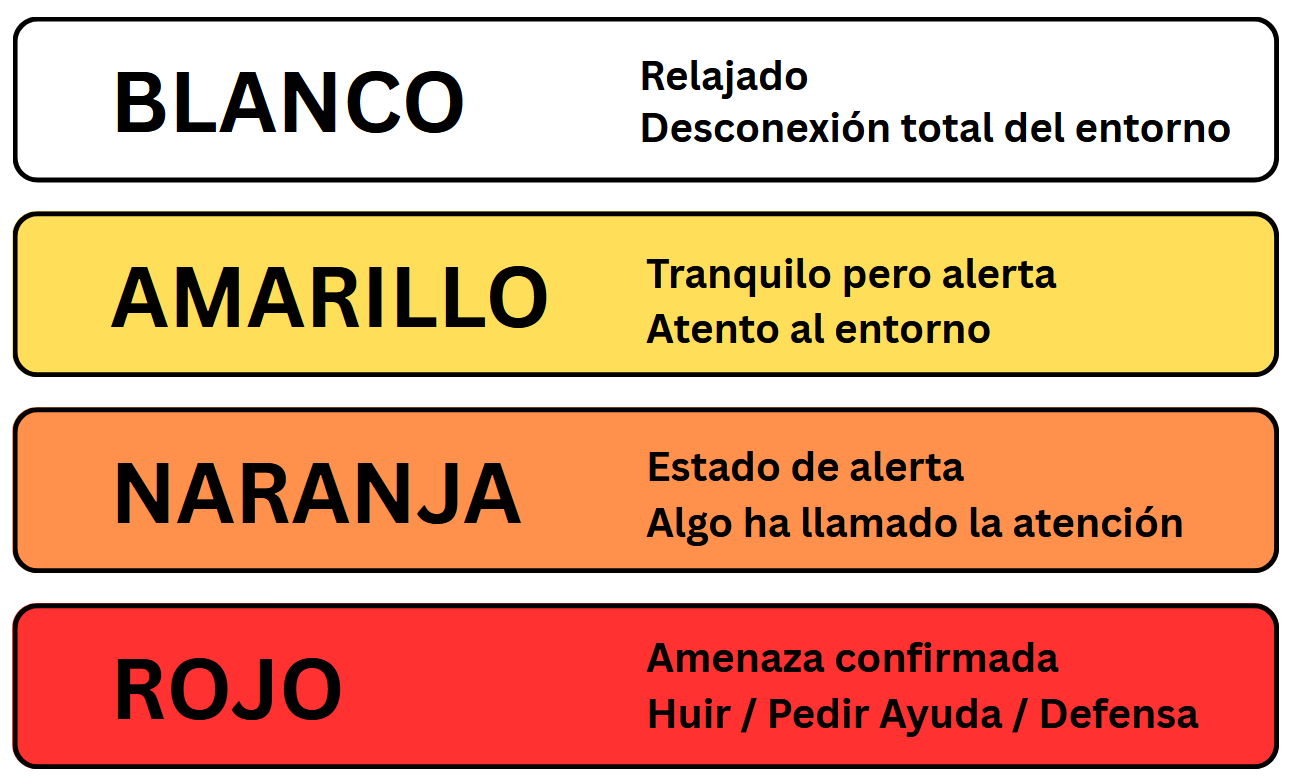
\includegraphics[width=\linewidth]{figures/cooper.png}

\section{La intuición es información}

La sensación de incomodidad o de \enquote{algo no va bien} ante una persona o lugar es un mecanismo de detección de señales reales que procesamos sin darnos cuenta (Gavin de Becker la describe en profundidad en su obra \emph{El valor del miedo}, \citeyear{debecker1997}). No la racionalices por cortesía: cambia de acera, no subas a ese ascensor, sal de ese portal. La educación social nos entrena para no \enquote{ofender}; \textbf{tu seguridad es más importante que la opinión de un desconocido}.

\section{Las tres distancias del conflicto}

\textbf{1) Distancia preventiva:} es la ideal para la defensa personal, ya que permite evitar el conflicto y no produce consecuencias. Si de noche debo pasar por un parque poco iluminado donde es común que se robe, hacer un rodeo por una calle iluminada y transitada me evita el riesgo. La defensa personal no se refiere solo a peleas: si evito esperar el metro muy cerca de las vías, estoy previniendo que alguien pueda empujarme (de manera intencionada o accidental).

\textbf{2) Distancia verbal o de negociación:} se establece cuando ya estamos inmersas en un conflicto. Todavía existe la posibilidad de disuadir al oponente y salir sin consecuencias. Lo siguiente en ocurrir suele depender en parte de los estímulos que lleguen al agresor.

\textbf{Debemos:}
\begin{itemize}
  \item Buscar la conciliación cuando el conflicto sea de baja intensidad (discusión, malentendido), intentando llegar a un acuerdo.
  \item Recordar al agresor las consecuencias (pérdida de tiempo o de prestigio, dolor, riesgo de ser detenido). Usar la técnica asertiva del \enquote{disco rayado}: repetir el mismo límite con las mismas palabras, sin entrar en provocaciones.
  \item Marcar límites con frases cortas, directas, en tono fuerte y con lenguaje corporal firme: \enquote{¡Para! ¡No te acerques!}. Verbalizar en voz alta también alerta a posibles testigos y rompe el guion del agresor, que espera una víctima callada.
\end{itemize}

\textbf{No debemos:}
\begin{itemize}
  \item Burlarnos, reírnos o ridiculizar al agresor.
  \item Insultarle.
  \item Iniciar el enfrentamiento con el lenguaje corporal.
  \item Sostener la mirada fija en los ojos de forma desafiante (sí mantenerlo en el campo visual).
  \item Tocar al agresor.
  \item Ignorarle por completo.
\end{itemize}

\textbf{3) Distancia física o de contacto:} puede llegar sin pasar por la distancia verbal, pero si deriva de esta, ya debemos haber recogido información del medio: cantidad de atacantes, vías de escape, elementos que puedan servir para la defensa, existencia de testigos, estado emocional del oponente, puntos vulnerables, etc.

\newpage

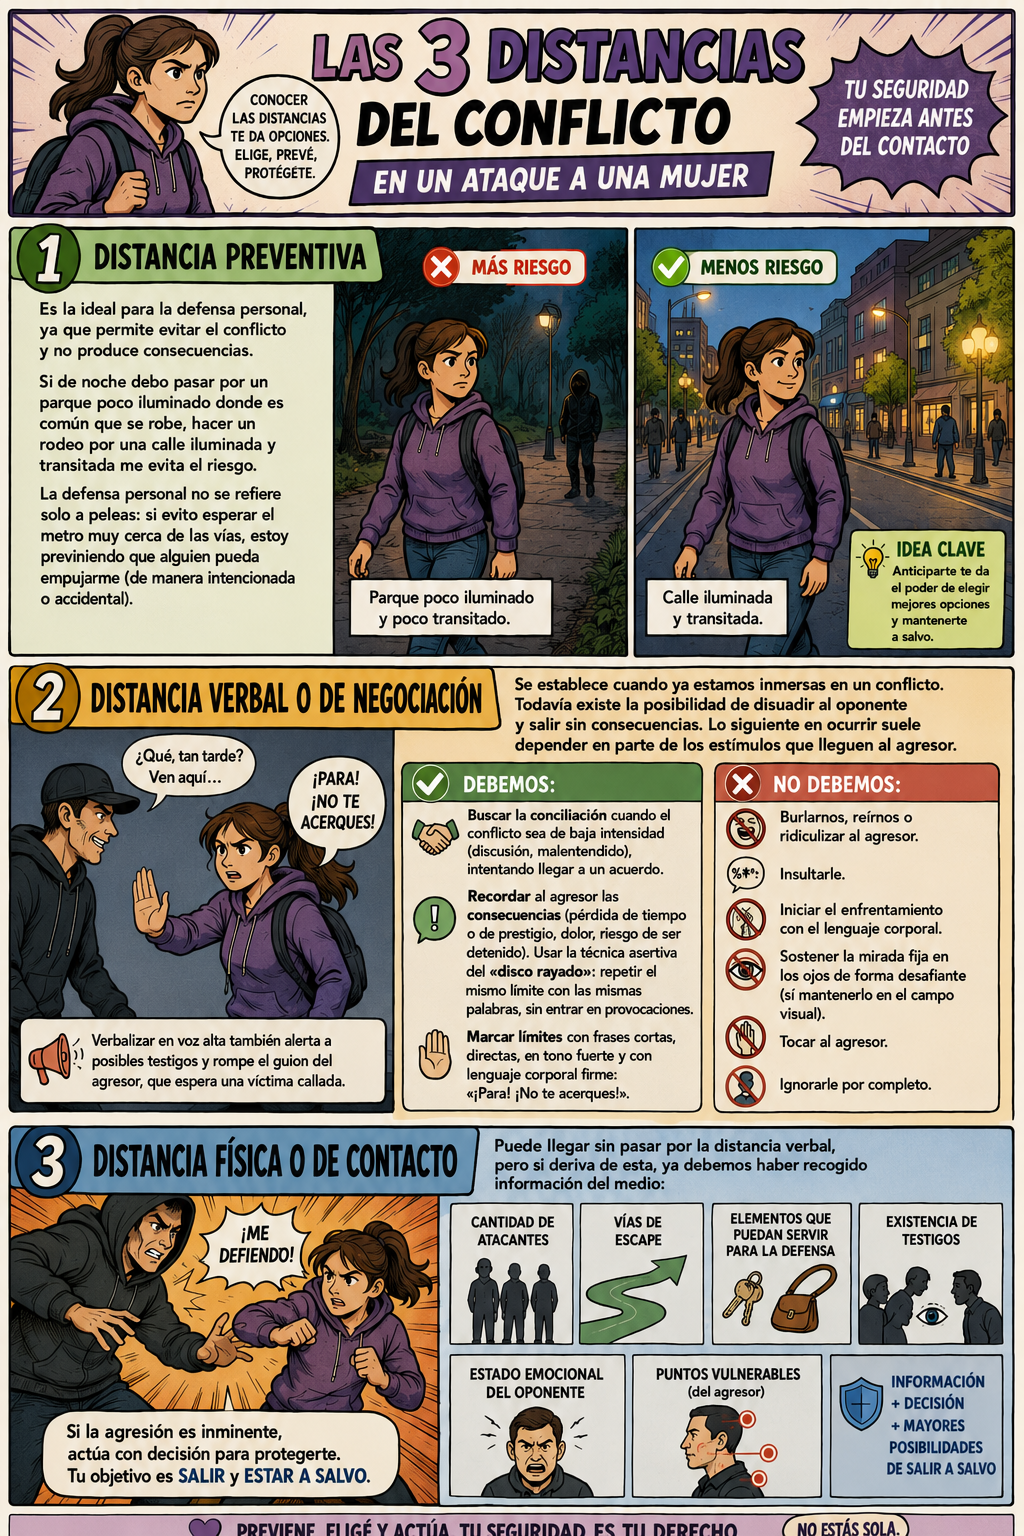
\includegraphics[width=\linewidth]{figures/tres-distancias.png}
